% ---------- עמוד שער ----------
\begin{titlepage}
\begin{tikzpicture}[remember picture, overlay]
  % רקע כחול-לילה
  \fill[night] (current page.south west) rectangle (current page.north east);
  % איור הרשת (נוצר ב-Python)
  \node[anchor=center, opacity=0.95] at ($(current page.center)+(0,1.2)$)
       {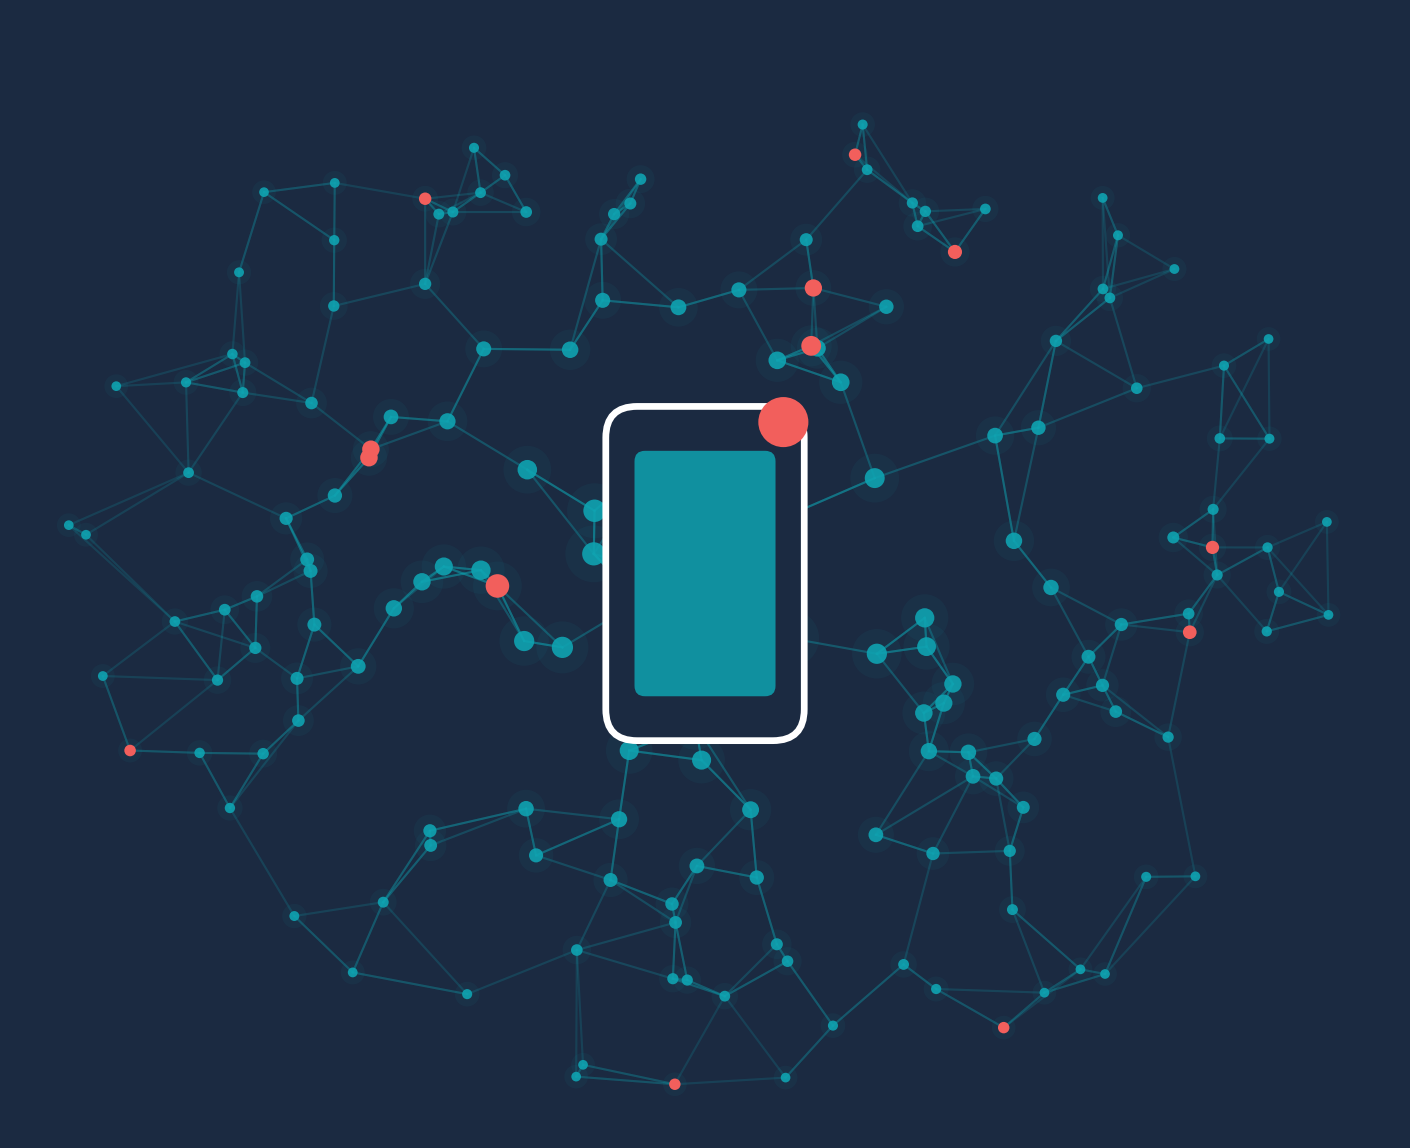
\includegraphics[width=\paperwidth]{images/cover_network.png}};
  % פס טורקיז
  \fill[screen] ($(current page.south west)+(0,4.2)$) rectangle ($(current page.south east)+(0,4.45)$);
  % כותרת
  \node[text=white, font=\headfont\bfseries\fontsize{48}{52}\selectfont, align=center]
       at ($(current page.north)+(0,-4.2)$) {\RL{מחוברים תמיד}};
  \node[text=screen, font=\headfont\fontsize{20}{24}\selectfont, align=center]
       at ($(current page.north)+(0,-5.7)$) {\RL{טכנולוגיה וחיי היומיום}};
  % נקודת התראה
  \fill[notif] ($(current page.north)+(5.6,-3.0)$) circle (0.35);
  \node[text=white, font=\headfont\bfseries\small] at ($(current page.north)+(5.6,-3.0)$) {\LR{9}};
  % פרטים בתחתית
  \node[text=white, font=\headfont\large, align=center]
       at ($(current page.south)+(0,2.9)$) {\RL{ספר שנכתב ב-\LR{LaTeX} בעזרת צוות סוכני בינה מלאכותית}};
  \node[text=white!70, font=\headfont, align=center]
       at ($(current page.south)+(0,2.0)$) {\RL{שנהב סולימאן \quad|\quad 2026}};
\end{tikzpicture}
\end{titlepage}
